\chapter{Конструкторская часть}

\section{Схемы алгоритмов}

Время выполнения стандартного алгоритма не зависит от каких-либо характеристик взржныхх матриц, из-за чего рассматривать лучший и худший случай будеи излишне.

В случае алгоритма Винограда стоит выделить 2 класса эквивалентности: четное и нечетное количество столбцов левой матрицы.

На рисунке 2.1 приведена схема стандартного алгоритма умножения матриц.

На рисунках 2.2 и 2.3 представлена схема алгоритма Винограда и схема оптимизированного алгоритма Винограда. 

\begin{figure}[ht!]
	\centering
	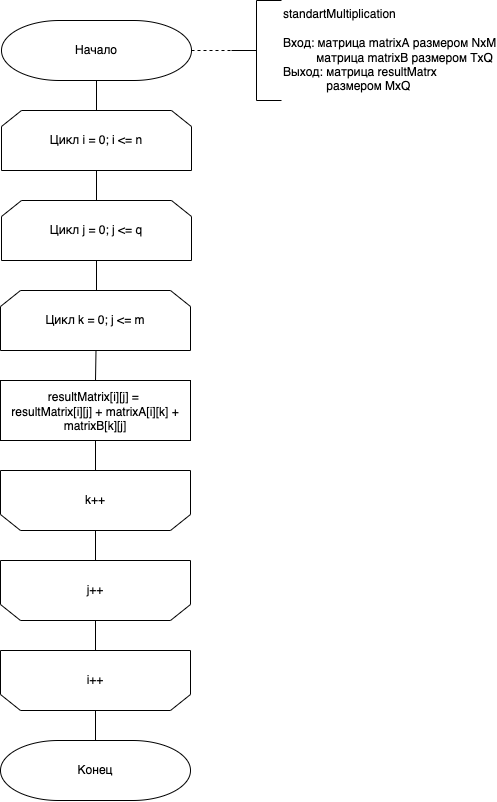
\includegraphics[width=0.9\linewidth]{img/Standard.png}
	\caption{Схема стандартного алгоритма умножения матриц}
	\label{fig:mpr}
\end{figure}

\begin{figure}[ht!]
	\centering
	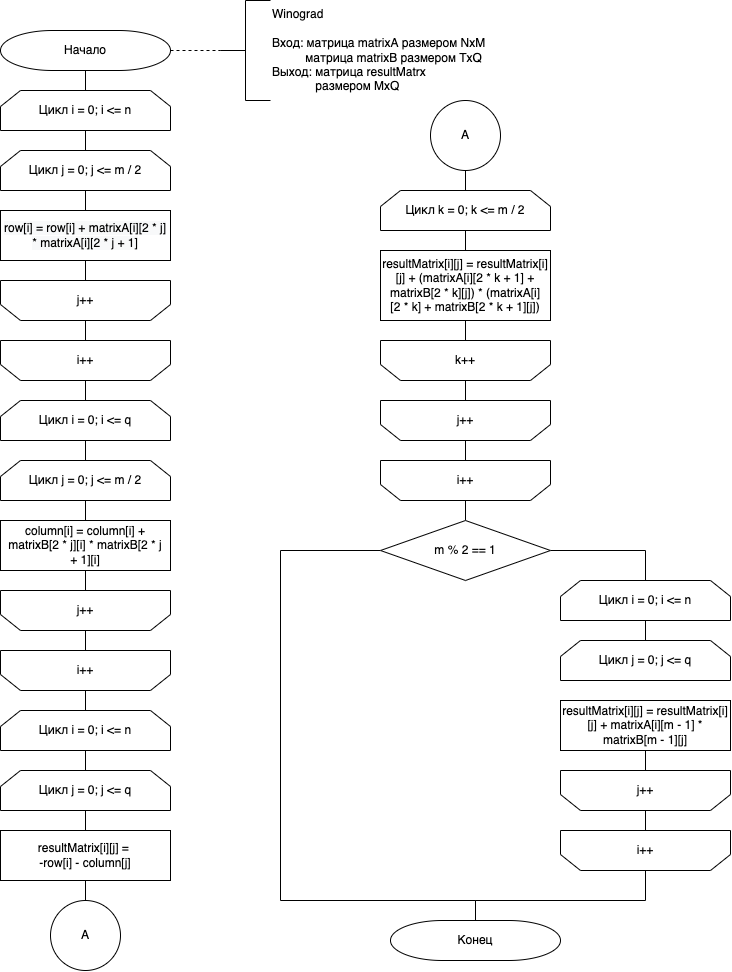
\includegraphics[scale=0.65]{img/Winograd.png}
	\caption{Схема алгоритма Винограда}
	\label{fig:mpr}
\end{figure}

\begin{figure}[ht!]
	\centering
	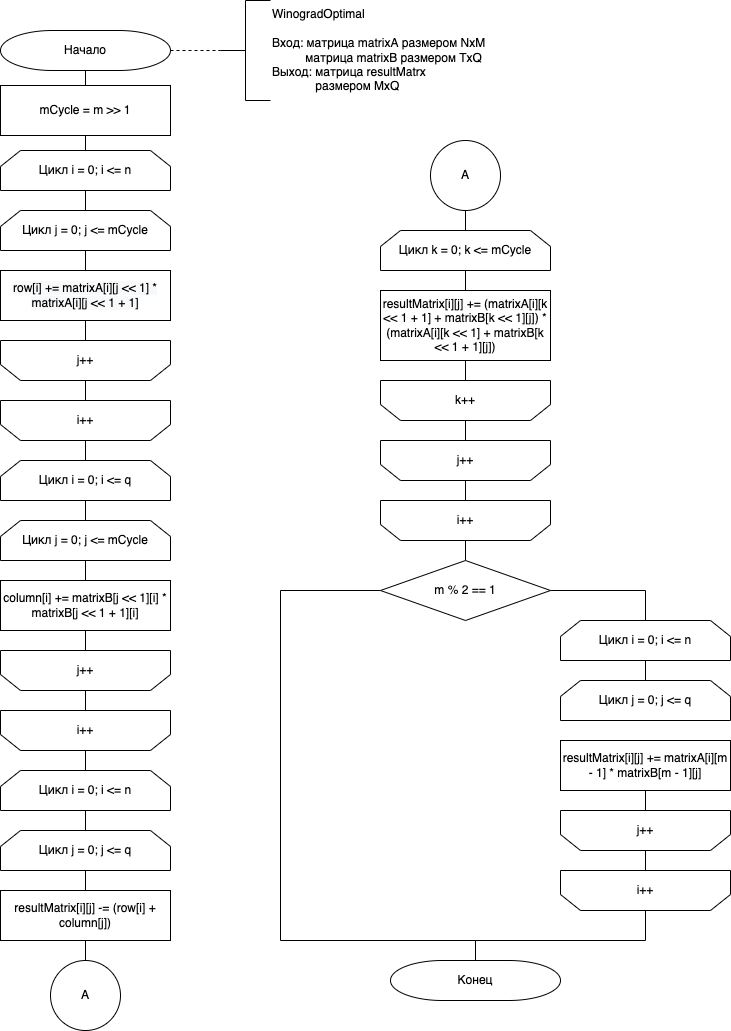
\includegraphics[scale=0.65]{img/WinogradOptimal.png}
	\caption{Схема функций оптимизированного алгоритма Винограда}
	\label{fig:mpr}
\end{figure}

\newpage

\section{Модель вычислений}

Для последующего вычисления трудоемкости введём модель вычислений.

\begin{enumerate}
	\item Операции из списка (\ref{for:opers}) имеют трудоемкость 1.
	\begin{equation}
	\label{for:opers}
	+, -, \%, ==, !=, <, >, <=, >=, [], ++, {-}-
	\end{equation}
	\item Операции из списка (\ref{for:opers_2}) имеют трудоемкость 2.
	\begin{equation}
	\label{for:opers_2}
	*, *=, /, /=
	\end{equation}
	\item Трудоемкость оператора выбора if условие then A else B рассчитывается по формуле (\ref{for:if}).
	\begin{equation}
	\label{for:if}
	f_{if} = f_{\text{условия}} +
	\begin{cases}
	f_A, & \text{если условие выполняется,}\\
	f_B, & \text{иначе.}
	\end{cases}
	\end{equation}
	\item Трудоемкость цикла рассчитывается по формуле (\ref{for:for}).
	\begin{equation}
	\label{for:for}
	f_{for} = f_{\text{инициализации}} + f_{\text{сравнения}} + N(f_{\text{тела}} + f_{\text{инкремента}} + f_{\text{сравнения}})
	\end{equation}
	\item Трудоемкость вызова функции равна 0.
	\item Трудоемкость выделения произвольного блока памяти на куче равна 10.
\end{enumerate}

\section{Трудоёмкость алгоритмов}

\subsection{Стандартный алгоритм умножения матриц}

\begin{enumerate}
	\item Трудоёмкость проверки на коррестность рамеров перемножаемых матриц составляет:
	\begin{equation}
	f_{check} = 1
	\end{equation}
	
	\item Трудоёмкость создания матрицы:
	\begin{equation}
	f_{create} = 10
	\end{equation}
	
	\item Трудоёмкость 1 цикла составляет:
	\begin{equation}
	\label{for:MV}
	f_{c1} = 1 + 2m + m \cdot f_{c2}
	\end{equation}

	\item Трудоёмкость 2 цикла составляет:
	\begin{equation}
	\label{for:MV}
	f_{c2} = 1 + 2l + l \cdot f_{c3}
	\end{equation}

	\item Трудоёмкость 2 цикла составляет:
	\begin{equation}
	\label{for:MV}
	f_{c3} = 1 + 2n + n \cdot 9
	\end{equation}
\end{enumerate}

Таким образом получим, что согласно введенной модели трудоемкость стандартного алгоритма составит:
$$
f_{standart} = 12 + 3m + 3ml + 11mnl = O(mnl)
$$

\subsection{Алгоритм Винограда}

\begin{enumerate}
	\item Трудоёмкость проверки на коррестность рамеров перемножаемых матриц составляет:
	\begin{equation}
		f_{check} = 1
	\end{equation}
	
	\item Трудоёмкость создания матрицы:
	\begin{equation}
		f_{create} = 10
	\end{equation}

	\item Трудоемкость подсчета сумм (предвычисление) для строк левой матрицы:
	\begin{equation}
		f_{row-factors} = 1 + 3m + 10mn
	\end{equation}
	
	\item Трудоемкость подсчета сумм (предвычисление) для столбцов правой матрицы:
	\begin{equation}
	f_{column-factors} = 1 + 3n + 10nl
	\end{equation}
	
	\item Трудоемкость выполнения основного цикла:
	\begin{equation}
	\label{for:impr_cycle}
	f_{cycle} = 9mnl + 8mn + 2m + 2
	\end{equation}

	\item Трудоемкость выполнения цикла при нечетном количестве строк второй матрицы:
	\begin{equation}
	\label{for:impr_cycle}
	f_{cycle} = 11ml + 3m + 3
	\end{equation}
\end{enumerate}

Для худшего случая имеем:
\begin{equation}
\label{for:bad_impr}
f_{va-best} = 16 + 5m + 3n + 18mn + 13 ml + 11nl + 9mnl = O(mnl)
\end{equation}

Для лучшего случая имеем:
\begin{equation}
\label{for:good_impr}
f_{va-best} = 16 + 5m + 3n + 18mn + 11nl + 9mnl = O(mnl)
\end{equation}


\subsection{Оптимизированный алгоритм Винограда}

Трудоемкость оптимизированного алгоритма винограда рассчитывается аналогично обычному алгоритму винограда и составляет:

\begin{equation}
	\label{for:good_impr}
	f_{va-best} = 16 + 5m + 3n + 15mn + 10nl + 8mnl = O(mnl)
\end{equation}

\section*{Вывод}
На основе теоретических данных, полученных из аналитического раздела, построены схемы алгоритмов умножения матриц.  Оценены их трудоёмкости в лучшем и худшем случаях.
